\documentclass[11 pt,russian]{article}
\hoffset=-2cm \voffset=-2.5cm \textwidth=17cm \textheight=23cm

\usepackage[utf8]{inputenc}
\usepackage[russian]{babel}
\usepackage{amssymb, amsfonts, amsthm, amsmath}
\usepackage{graphicx}
\DeclareGraphicsRule{*}{mps}{*}{}

\newcounter{variant}
\newcounter{zadacha}[variant]

\newcommand{\z}{\par\addtocounter{zadacha}{1}%
\textbf{\arabic{zadacha}.}\ }

\newcommand{\var}{\par\addtocounter{variant}{1}%
\textbf{Вариант \arabic{variant}.}\\}

\newcommand{\mymp}[1]{\begin{minipage}{0.5\textwidth}#1\end{minipage}}


\theoremstyle{plain}
\newtheorem{theorem}{Теорема}
\newtheorem{lemma}{Лемма}
\newtheorem{corollary}{Следствие}
\newtheorem*{theorem*}{Теорема}
\newtheorem*{lemma*}{Лемма}
\newtheorem*{corollary*}{Следствие}

\theoremstyle{definition}
\newtheorem{definition}{Определение}
\newtheorem{example}{Пример}
\newtheorem{remark}{Замечание}
\newtheorem*{definition*}{Определение}
\newtheorem*{example*}{Пример}
\newtheorem*{remark*}{Замечание}

\newtheorem*{task}{Задача}
\newtheorem*{task*}{Задача}

\newcommand{\Answer}[1]{\vspace{-0.3cm}Ответ: #1.}

%\renewcommand\qedsymbol{$\blacksquare$}
\renewcommand{\leq}{\leqslant}
\renewcommand{\geq}{\geqslant}

%=============================================

\begin{document}

\vspace{1cm}
\hrule
\vspace{1cm}

\begin{figure}[h]
\center{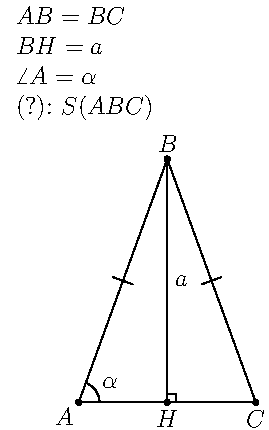
\includegraphics[scale =1.0]{pic.pdf}}
\end{figure}


\begin{proof}[Решение]\ 
\begin{enumerate}
\item В $\triangle ABH$: $\tg\angle A =\dfrac{BH}{AH}$. Следовательно: $AH=\dfrac{BH}{\tg\angle A}=\dfrac{a}{\tg\alpha}$
\item По свойству высоты в равнобедренном треугольнике, высота является медианой. Тогда:
$$
AH=HC=\dfrac{a}{\tg\alpha}\rightarrow AC=AH+HC=\dfrac{2a}{\tg\alpha}
 $$
\item По формуле площади для треугольника получаем:
$$
S(ABC)=\dfrac{1}{2}\cdot BH\cdot AC=\dfrac{1}{2}\cdot\dfrac{2a}{\tg\alpha}\cdot a=\dfrac{a^2}{\tg\alpha}=a^2\cdot\ctg\alpha
$$

\end{enumerate}

\end{proof}
\Answer{$S(ABC)=a^2\cdot\ctg\alpha$}

\end{document}

